\documentclass{beamer}
\usetheme{Boadilla}

\usepackage{amsmath}
\usepackage{amsfonts}
\usepackage{amssymb}
\usepackage{tikz}

\title{My Beamer Example}
\author{My Name}
\institute{My Home Institution}
% I normally would use \date{\today}. I wrote out the date instead so that if
%  you compile it on a different day it still looks like the example pdf
\date{June 2, 2017}

\begin{document}

	% Your first slide should always be a title slide
	\begin{frame}
		\maketitle
	\end{frame}
	
	\begin{frame}{Tables}
		Let's make a simple table for boolean logic.
		% We will start in the center environment to center our table
		\begin{center}
			% tabular takes an argument telling it how many columns and the formatting of the columns
			% c: center aligned column
			% l: left-aligned column
			% r: right-aligned column
			% placing a | (shift+\) places a verticle line in the table 
			%               in the same place relative to the columns
			\begin{tabular}{c|c||c|c}
				% Use & to tell tabular you are moving to the next
				%                                 column of your row
				X & Y & X AND Y & X OR Y \\
				% \hline makes a horizontal line at the top of your current row
				\hline
				T & T &    T    &    T   \\
				T & F &    F    &    T   \\
				F & T &    F    &    T   \\
				F & F &    F    &    F
			\end{tabular}
		\end{center}
		
		Matrices can be built in a similar manner, but you must be in math mode
		\begin{center}
			$
			\begin{bmatrix}
			0    &   1    & \hdots &   2    \\
			3    &   4    & \hdots &   5    \\
			\vdots & \vdots & \ddots & \vdots \\
			6    &   7    & \hdots &   9
			\end{bmatrix}
			$
		\end{center}	
	\end{frame}	
	
	% the argument after the frame gives the slide a title
	\begin{frame}{Lists}	
		We can make an itemized list:
		\begin{itemize}
			\item This list
			\item will display
			\item all at once
		\end{itemize} 
		
		We can also make enumerated lists:
		\begin{enumerate}
			% \pause makes the presentation wait for you to prompt it 
			%                        before displaying what comes next
			\pause
			\item We will show 
			\pause
			\item only one entry 
			\pause
			\item at a time
		\end{enumerate}
	\end{frame}
	
	
	% Add an argument to the frame environment to give your slide a title
	\begin{frame}{Definition Blocks}
		\begin{definition}
		A \textbf{right triangle} is a triangle in which one of the angles is a right angle. The side opposite of the right angle is called the \textbf{hypotenuse} and the other two sides are called \textbf{legs}.
		\end{definition}
		
		% the figure environment will center our picture, use internal logic to 
		% move it to a visually appealing place, make it easy to add a caption, 
		% and is often used in papers to more easily cite drawings and make a 
		% table of diagrams
		%     The [optional tag] is used to tell LaTeX where it should try to %      place the picture. h=here, t=top, b=bottom, etc.
		\begin{figure}[hb]
			% Use tikz to draw a right triangle
			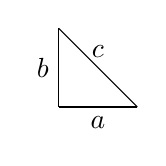
\begin{tikzpicture}
				%the node command here allows us to place a label along the line
				\draw (0,0) -- (1,0) node[midway, below] {$a$}; 
				\draw (0,0) -- (0,1) node[midway, left] {$b$};
				\draw (1,0) -- (0,1) node[midway, above] {$c$};
			\end{tikzpicture}
			\caption{A right triangle (No need to TeX this! Ola will explain how to use TikZ later)}
		\end{figure}
	\end{frame}
	

	\begin{frame}{Theorems and Figures}
		% The [optional tag] names the theorem
		\begin{theorem}[The Pythagorean Theorem]
			The sums of the squares of the legs of a right triangle is equal to the square of its hypotenuse. In reference to the labels in the previous figure, this may be written as $a^2 + b^2 = c^2$
		\end{theorem}
		\pause 
		% You can also use an optional tag to replace "Proof" with a more 
		%     accurate description, e.g. "Sketch of Proof"
		\begin{proof}
			% The picture we are using is quite large, so we use an optional 
			%  argument to rescale it. There are many different ways to do this
			\includegraphics[height=.4\textheight]{pythag_proof.jpg}
		\end{proof}
	\end{frame}
	
	
	
	\begin{frame}{Advanced Topic- The Columns Environment}
		The columns environment splits your page up into multiple columns of content.
                
                \vspace{0.3in}

		% Split into columns now
		\begin{columns}
			% start first column and give how wide it is
			\begin{column}{0.4\textwidth}
				Equation 1 \\
				% Our first diagram is simple enough to write using 
				%      standard math packages
				\[ (a + b) (a - b) = a^2 - b^2 \]
			\end{column}
			% start second column
			\begin{column}{0.4\textwidth}
				Equation 2 \\
                                $$ (a - b) (a^2 + ab + b^2) = a^3 - b^3 $$
			\end{column}
		\end{columns}

                \vspace{0.3in}
			
		Columns is also a nice environment for placing equations and graphs side-by-side.		
	\end{frame}
	

\end{document}
